% Chapter 1

\chapter{Datasets} % Write in your own chapter title
\label{Chapter3}
\lhead{Chapter 3. \emph{Datasets}} 
\section{Kinetics-600}
The \textbf{Kinetics-600} \cite{kinetics-600} is an action recognition dataset that consists of approximately 500K videos from 600 action categories each containing at least 600 videos. Each video in the dataset is a 10-second clip of an action moment from a YouTube video. This was an extension of the Kinetics-400 \cite{kinetics-400} dataset. The goal of the Kinetics project was to replicate 1000 classes, each with 1000 image examples like in ImageNet.

There were two main bottlenecks in the Kinetics-400 dataset: 

(i) Identifying relevant candidate YouTube videos for each action class

(ii) Find classes with many candidates. 

The last 10 seconds of YouTube videos were taken as clips. They had a variable resolution and frame rate. For the action class, all clips were taken from different YouTube videos. In this dataset, the number of classes has increased by 50\%, from 400 to 600, and the number of video clips has increased by 60\%, from approximately 300k to approximately 500k.

Although the dataset has 600 classes of activities, it does not have the exact activities that we require for our application. It contains a few activities somewhat similar to the ones we would like to detect such as we want to detect talking which exists as “talking on a cell phone.” For eating it has classified the activity based on different foods, such as spaghetti, carrots, burger, chips, ice cream, hotdog, watermelon, doughnuts, and cake. For a person walking, the dataset refers to the activity of walking a dog or walking with a horse. For fall detection, it addresses only falling from a chair or falling from a bike but the latter is not of use to us. The only activity that may match our use case is the sleeping activity which is included in the dataset. 

 The dataset was split into 392,622 clips that were used for training, 30000 for validation, and 60000 for testing. The clips unlike in Kinetics-400 do not contain multiple activities such as “texting” while “Walking” as the data collection methodology changed removing such anomalies. The data collection process is as follows:

 As in Kinetics-400 a class list for human actions was decided using multiple sources such as past action datasets, motion capture datasets, and crowd-sourcing systems such as Amazon Mechanical Turk (AMT). The key difference with the Kinetics-600 datasets is that many classes were sourced from Google’s Knowledge Graph and YouTube’s search box auto-complete; for example, an object or a verb was typed and auto-complete suggestions were followed up to see if they contained enough videos of the same action to decide whether or not that class would be a part of the dataset. For the Kinetics-400 dataset video titles were matched with action lists. Image classifiers extracted the clips where an activity was detected. Every clip used originated from a different YouTube video. AMTs then labeled the clips and identified whether a specific action was occurring in the clip's duration. Only the clips with 3/5 positive responses were added to the dataset. For the Kinetics-600 dataset, a set of queries was prepared for each class in the two most spoken languages, English and Portuguese. As an example, the queries for the folding paper were: “folding paper” (en), “origami” (en), and “dobra papel” (pt). Instead of matching the textual queries directly weighted n-gram representations of the combination of the metadata of each video and the titles of related videos were used. Combined, with standard title matching, a robust similarity score between a query and all YouTube videos was obtained.
The dataset was then cleaned up in the last stage. Duplicates were removed from the dataset by comparing the similarity score between feature vectors. Noisy classes were either merged or removed. Final filtering was performed by sorting examples in decreasing order of confidence. The dataset file contained a field named “label”, YouTube ID, time start and time end (in seconds), and "split" that identified whether the sample was for testing, training, or validating data.
\section{Kinetics 700}
After Kinetics-600, the Kinetics-700 \cite{kinetics-700} dataset was released comprising 700 action classes, each with at least 700 video clips. From the dataset, 545793 clips are used for training, 35000 for validation, and 70000 for testing.  Synonyms and searches in different languages i.e. English, French, Spanish, and Portuguese are used to get more clips for the rarest classes. Duplicate clips are removed by clustering the clips. The dataset contains a label that indicates the activity performed, YouTube ID time and start and time end (in seconds), and split to tell if it is testing, training, or validating data.  
\section{Toyota Smart Home Dataset}
The Toyota Smarthome dataset was captured in a residence with seven Kinect v1 cameras. It comprises 31 activities of daily living of 18 senior citizens between the ages of 60 and 80. The activities are recorded in 3 different scenes from 7 camera viewpoints. Each person is recorded for 8 hours in one day from morning until the afternoon. The dataset has a 640x480 resolution and three modalities: RGB, Depth, and 3D Skeleton. RGB was used to extract the 3D skeletal joints. The persons' faces are blurred for privacy concerns. The dataset is available in two versions: Trimmed Toyota Smarthome \cite{Das_2019_ICCV} and Untrimmed Toyota Smarthome (TSU) \cite{dai2022toyota}. We use the untrimmed dataset version, and particularly the Balanced Untrimmed dataset to train our forecasting model.
\begin{figure}[h]
    \centering
    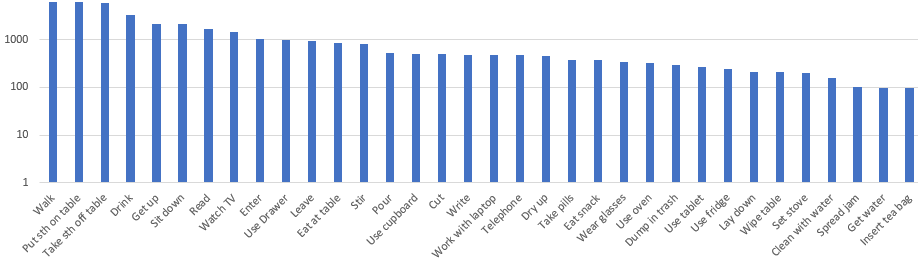
\includegraphics[width=0.8\textwidth]{images/Balanced_TSU.PNG}
    \caption{Activities Involved in Balanced Untrimmed Dataset}
    \label{fig:balancedtsu}
\end{figure}
The original Toyota untrimmed smart home video dataset has close to 51 actions and the frequency of the occurrence of these actions in the videos is highly unbalanced which means that certain actions occur more frequently than others. Therefore, certain low-frequency actions were removed and a final balanced dataset consisting of only 34 highly occurring actions was created. Balanced TSU shares the same untrimmed videos as fine-grained TSU: 536 videos with 21 21-minute average duration. Activities were carried out in a highly spontaneous way. The activities involved in the Balanced Untrimmed dataset are shown in figure \ref{fig:balancedtsu}. The activities that are within the project's scope are: \\
Walk, drink, get up, sit down, take pills, eat, eat a snack, read, watch TV, leave, lay down.

\section{THUMOS14}
The \cite{thumos-14} dataset serves as a cornerstone for training the Boundary Sensitive Network (BSN) for temporal action proposal generation. THUMOS14 is a comprehensive dataset specifically designed for temporal action localization tasks. It contains over 254 hours of video data across 101 action classes. It has annotated splits, including training, validation, background, and test sets. THUMOS14 provides a robust platform for evaluating the effectiveness of action recognition algorithms. The dataset offers spatio-temporal annotations and pre-extracted features, enhancing its utility for training and testing various models. THUMOS14 remains a widely adopted standard in the field due to its extensive content and well-defined evaluation protocols, making it an ideal choice for training the BSN model in this study.

The dataset boasts meticulous curation and annotation, ensuring its suitability for training and evaluating action localization algorithms. With over 254 hours of video data, comprising approximately 25 million frames, THUMOS14 offers a substantial corpus for temporal action localization tasks. This dataset is carefully categorized into distinct splits, including a comprehensive training set with over 13,000 temporally trimmed videos covering 101 action classes, a validation set featuring over 1,000 untrimmed videos with temporal annotations, and a background set containing over 2,500 videos devoid of any of the 101 action classes to prevent false positives. The test set comprises 1,500 untrimmed videos with withheld ground truth labels, allowing researchers to benchmark their models' performance on unseen data. The data collection process for THUMOS14 involved sourcing videos from YouTube reflecting real-world scenarios and ensuring the dataset's relevance and applicability to practical action recognition tasks. THUMOS14's well-defined evaluation protocols encompass a range of metrics tailored to assess temporal action proposal generation algorithms' performance accurately. The protocols include metrics such as mean Average Precision (mAP) and Intersection over Union (IoU), providing researchers with clear guidelines for assessing and comparing the efficacy of different models trained on the dataset.

\section{AVA-Kinetics}
The AVA-Kinetics dataset \parencite{ava-kinetics} is a comprehensive video dataset focused on human actions. It merges the AVA dataset and the Kinetics-700 dataset by applying AVA-style annotations to Kinetics-700 videos. The AVA dataset includes 80 different actions across 430 video clips, each lasting 15 minutes. Annotating the AVA dataset is costly because it involves marking actions for each person in a video clip at a one-second interval. It also involves generating a bounding box around each individual to assign multiple concurrent activity labels. The dataset is divided into 141,475 clips for training, 32,592 clips for validation, and 64,902 clips for testing.
Initially, a pre-trained Faster RCNN detects the frame with the individuals and highest detection score. Human annotators then add any missing bounding boxes in the data. A 2-second video segment centered around this keyframe is extracted, and at least three human raters propose action labels for the person in that keyframe. These labels are later verified by two to three additional raters.
The dataset includes 27 AVA classes with low recognition accuracy and 115 related classes from the Kinetics dataset. The dataset file contains several details: a video ID (identifier on YouTube), the timestamp of the middle frame (in seconds from the video's start), the bounding box coordinates of the person (x1, y1, x2, y2), an action ID for the performed action, and an optional person ID linking bounding boxes if depicting the same individual. 

\section{ImageNet}
The ImageNet dataset \parencite{image-net} stands as a monumental cornerstone in computer vision research, constituting a vast image database structured according to the WordNet hierarchy. With an ambitious goal to furnish approximately 1,000 meticulously annotated images for each synset in WordNet, ImageNet boasts tens of millions of meticulously labeled images encapsulating a diverse spectrum of concepts. Its inception stemmed from the imperative to address two critical exigencies in the field: firstly, establishing a quintessential benchmark task for computer vision—the North Star Problem—choosing object categorization as the central challenge, and secondly, mitigating the paucity of data requisite for fostering generalizable machine learning methodologies, especially in light of the burgeoning digital data landscape. While the precise methodologies employed for image collection remain undisclosed to the public, it is inferred that images were procured from myriad online sources, likely through web searches and image scraping, with a rigorous quality control mechanism ensuring image fidelity. Human annotators meticulously categorized images into their corresponding synsets, augmenting an automated process that handled the sheer scale of data. The profound impact of ImageNet on computer vision research, particularly in catalyzing advancements in deep learning, cannot be overstated. Deep convolutional neural networks, pivotal to contemporary breakthroughs, owe a debt to ImageNet's extensive labeled data. Nevertheless, contemporary discourse has surfaced criticisms regarding potential biases and limitations within the dataset, stimulating a quest among researchers for more inclusive and expansive datasets to propel the field forward.

\section{ActivityNet-1.3}
Many existing datasets are quite basic. In contrast, the ActivityNet dataset \parencite{activity-net} is a comprehensive, video-based dataset that encompasses a wide array of intricate activities. It comprises 203 activity classes, each class having an average of 137 untrimmed videos. On average each video contains 1.41 instances of activities, making up a total of 27,801 videos and 849 hours of footage. This dataset is the first extensive human activity database to categorize a substantial number of videos using a semantic taxonomy. Crafting a semantic framework for activities is complex, so this dataset utilizes the Department of Labor's activity taxonomy from the American Time Use Survey. It contains over 2000 activities out of which only 203 activity categories were chosen. Activity classes are organized into seven top-level categories: Personal Care, Eating and Drinking, Household, Caring and Helping, Working, Socializing and Leisure, and Sports and Exercises.

The data collection process follows several stages. Initially, videos are sourced from YouTube by searching for specific activity labels. These videos are then verified by Amazon Mechanical Turk, who ensure that each video contains the intended activity. Non-compliant videos are excluded.  Only experienced workers are employed to ensure integrity. Turkers then manually annotate the segments of the videos where the desired activities occur. A single video can include multiple activity labels. The dataset file contains labels, duration, start and end times (in seconds), the subset type, and a URL linking to the video on YouTube. 50\% of the dataset is used for training, 25\% for validation, and the remaining 25\% for testing.

\section{HACS}
The Human Action Clips and Segments (HACS) dataset \parencite{HACS} is designed for human action recognition in videos. Utilizing 200 action classes similar to those in ActivityNet. The dataset was compiled by querying YouTube with these labels, resulting in an initial collection of 890,000 videos. After removing duplicates, the dataset includes 504,000 clips, each averaging 2.6 minutes in length.
This dataset features two types of manual annotations. The first type involves action labels on 1.5 million 2-second clips extracted from the videos. These clips are included by comparing results from various visual classifiers. The second type, HACS Segments, focuses on temporal localization within 50,000 untrimmed videos, ensuring each video contains at least one action segment. The segments in HACS are shorter in comparison to ActivityNet with 4.7 times more segments and 2.5 times more videos.
The dataset file includes: the class name, YouTube ID, a subset designation (training, validation, or testing), and start and end times (in seconds). A label of 1 denotes a positive sample, while -1 indicates a negative sample.
The authors have divided the dataset into a training set comprising 1.4 million clips sourced from 492,000 videos and a validation and testing set with 50,000 clips each.

\section{MMACT}
The MMACT dataset \parencite{MMAct} is a large-scale collection designed to improve action detection and recognition. It includes over 36,000 action instances across 37 classes, covering tasks like desktop activities and check-in procedures. The dataset features seven types of data modalities. Twenty subjects participated, wearing smart glasses for egocentric videos, carrying smartphones with sensors in their pants, and wearing smartwatches. The data was collected in four indoor settings: free space, occlusion areas, entrances, and desk work. Research shows the dataset is effective for studying actions across different subjects, scenes, views, and sessions. The MMACT dataset provides a diverse and detailed resource for action recognition studies.

\section{IKEA ASM}
IKEA ASM \parencite{IKEA} is a video dataset focused on assembly tasks. It aims to help analyze and understand human activities through actions, objects, and poses. The dataset includes 371 samples of furniture assembly with ground-truth annotations. Each sample features three RGB views, a depth stream, atomic actions, human poses, object segments, object tracking, and camera calibration data. Forty-eight participants assembled furniture in different locations: offices, labs, and homes. The data was collected using three Kinect V2 cameras placed to capture the work area from the front, side, and top. The dataset includes 16,764 annotated activities, with each action averaging 150 frames or 6 seconds.

\section{Home Action Genome}
The Home Action Genome dataset \parencite{home-action-genome} is used for action recognition in multi-view video databases of indoor activities. Data was collected from 27 participants in two houses, capturing diverse viewpoints for both low-level and high-level actions. The dataset includes recordings from 27 types of sensors, such as RGB cameras, infrared sensors, microphones, RGB lights, regular lights, accelerometers, gyroscopes, human presence detectors, magnets, air pressure sensors, humidity sensors, and temperature sensors. These sensors were placed in various locations around the houses and on participants' heads. The dataset provides three types of labels: video-level activity labels, temporally localized atomic activity labels, and spatio-temporal scene-graph labels. It includes annotations for 75 different activities.

\section{UR Fall}
UR-Fall consists of 70 sequences: 30 fall events and 40 daily living activities. Falls are recorded with two Microsoft Kinect cameras and an accelerometer. Daily living activities are captured using one camera (camera 0) and an accelerometer. Sensor data comes from PS Move (60Hz) and x-IMU (256Hz) devices. Each entry in the dataset includes sequences of depth and RGB images from cameras 0 and 1, which are placed on the floor and ceiling, respectively. It also contains synchronization and raw accelerometer data. Video streams are saved as PNG image sequences in separate zip files, with depth data in PNG16 format. 

\section{VidSitu}
VidSitu \parencite{VidSitu}  is a dataset designed for semantic role labeling in videos. It includes a large collection of video data with 29,000 movie clips, each 10 seconds long. Every 2 seconds of the clip is annotated with a verb and semantic roles. Entities are tracked across different events in the same clip. The events are linked through event-event relations. The clips are taken from a set of 3,000 videos and feature a variety of actions, with each video containing an average of 4.2 unique verbs.  200 verbs have more than 100 annotations each, making the dataset both complex and diverse.

\section{WISDM}
\cite{WISDM} "WISDM Smartphone and Smartwatch Activity and Biometrics Dataset" includes data from 51 subjects performing 18 different tasks for 3 minutes each. Data was collected using smartwatches and smartphones in controlled lab settings. Subjects engaged in activities such as walking, jogging, using stairs, sitting, standing, typing, clapping, and eating pasta. These activities fall into three categories: \\
(i) Activities not involving hands. (ii) General hand-focused activities. (iii) Eating-related hand activities\\
The accelerometer and gyroscope on both devices recorded raw time-series sensor data at a rate of 20Hz.  

\section{UCI-HAR}
The UCI-HAR \parencite{UCI-HAR} dataset records data from people wearing smartphones on their waists. These phones have two sensors. Thirty people aged 19-48 participated. Each person performed six activities: Walking, walking upstairs, walking downstairs, sitting, standing, laying.

The smartphone sensors are an accelerometer and a gyroscope. They record linear acceleration and angular velocity at 50Hz. A video captures the activities. Features are generated from the sensor data for the six activities. The dataset uses features from the accelerometer and gyroscope sensors. The acceleration signal is split into body and gravity signals using a Butterworth Filter. Jerk signals are also calculated.

\section{Opportunity}
The Opportunity \parencite{opportunity} dataset is designed to develop activity recognition algorithms using motion sensor data. It contains 2551 instances and 242 attributes. The dataset includes numerous activity instances and sensors of various types, simulating real-world data. It is also used for classification, automation segmenting, sensor selection, and feature selection.
Data was collected from three types of sensors: Body-worn sensors, object sensors, and ambient sensors
\end{enumerate}
Body-worn sensors have 145 attributes, object sensors have 60 attributes, and ambient sensors have 37 attributes. The setup includes 73 sensors with 10 modalities placed on the body, in the environment, and on objects. Subjects perform activities in a room with a deckchair, kitchen, door, coffee machine, chair, and table. Activities of daily living are recorded and synchronized with video footage.
Four people participate, each performing activities naturally and in scripted drills. The dataset includes 25 hours of data and is categorized into five tracks: Locomotion (e.g., sitting, standing), High-Level Activities, Left Arm movements and Right Arm movements.

\section{USC-HAD}
The UCS-HAD \parencite{USC-HAD} dataset is used to compare different algorithms in healthcare scenarios. It aids in creating a robust recognition system by training on a diverse group of people. Fourteen subjects, including 7 males and 7 females aged 21-49, participated. Their heights ranged from 160-185 cm, and their weights from 43-80 kg. The experiment involved the activities: Running, Jumping, Sitting, Standing, Walking,  Sleeping, Elevator Up, Elevator Down.
Each subject wore a mobile phone pouch at their front right hip with an embedded MotionNode. It is a motion-sensing application that sends data to a laptop. Subjects held a miniature device in one hand and performed 5 trials of activities on different days. The experiment was recorded and segmented based on start and end points noted by the observer. Each activity trial was saved in a separate file. The .mat file includes information such as height, weight, date, serial number, activity name, activity number, sensor location, orientation, and readings.

\section{Rose NTU}
The Rapid Rich Object Search lab has two datasets. One dataset includes 60 action classes and 56,880 RGB video samples. The activities fall into three categories: daily actions, mutual actions, and medical conditions. Each dataset is captured simultaneously by three Kinect V2 cameras. The RGB videos have a resolution of 1920x1080 pixels, while depth maps and infrared videos have a resolution of 512x424 pixels. The 3D skeletal data provides the 3D coordinates of 25 body joints in each frame. Examples of actions include: staggering, falling down, headache, chest pain, drinking water, standing up, sitting down, eating a meal, and opening a bottle.

\section{PAMAP2}
The PAMAP2 Physical Activity Monitoring \parencite{pamap} dataset is used for activity recognition and intensity estimation. This involves data processing, segmentation, feature extraction, and classification. The experiment includes 9 subjects wearing 3 inertial measurement units (IMUs) and a heart rate monitor. These subjects perform 18 activities, such as cycling, walking, and playing soccer. Each subject wears one IMU on the wrist, one on the chest, and one on the dominant ankle. The heart rate monitor samples data at 9 Hz. The dataset records the subjects performing these 18 activities.